\documentclass{article}
\usepackage[utf8]{inputenc}

\title{KREPE2 Battery Tabbing Process Specification and Acceptance Testing}
\author{Matt Ruffner, Kirsten Ford}
\date{}

\usepackage{url}
\usepackage{float}
\usepackage{tikz}
\usepackage{natbib}
\usepackage{graphicx}
\usepackage{listings}
\usepackage{subcaption}
\usepackage{fullpage}
\usepackage{hyperref}
\usepackage{pdfpages}
\hypersetup{
    colorlinks=true,
    linkcolor=blue,
    filecolor=magenta,      
    urlcolor=cyan,
}

\begin{document}

\maketitle
\tableofcontents
\listoffigures
\listoftables
\newpage


%%%%%%%%%%%%%%%%%%%%%%%%%%%%%%%%%%%%%%%%%%%%%%%%%%%%%%%%%%%%%%%%%%%%%%%%%%%%%%%%%%%%%%%%%
%%%%%%%%%%%%%%%%%%%%%%%%%%%%%%%%%%%%%%%%%%%%%%%%%%%%%%%%%%%%%%%%%%%%%%%%%%%%%%%%%%%%%%%%%
%%%%%%%%%%%%%%%%%%%%%%%%%%%%%%%%%%%%%%%%%%%%%%%%%%%%%%%%%%%%%%%%%%%%%%%%%%%%%%%%%%%%%%%%%
%%%%%%%%%%%%%%%%%%%%%%%%%%%%%%%%%%%%%%%%%%%%%%%%%%%%%%%%%%%%%%%%%%%%%%%%%%%%%%%%%%%%%%%%%
\section{Introduction}
This document outlines the procedures and verifications done to ensure the integrity of the spot welds used to attach tabs to the 18650 cells for the KREPE-2 mission. The procedures and specifications in this documents have been written to adhere to the guidelines of NASA battery tabbing and specification document \textit{\textbf{PRC-0009 Rev. D}}. According to this document, ``A Welding Procedure Specification (WPS) shall be qualified for each unique weld type to be produced by conforming to the requirements below, before the production welds are made." The WPS for tabbing the KREPE-2 batteries is defined in the following section. 


\section{Battery Acceptance Testing}

1 minute per axis

used spectrum that was already qualified by JSC document, help with reflight

Batteries were vibration tested at Yokohama facilities at the cell level on each axis. Capacity and open circuit voltage (OCV) were recorded before (see Tab. \ref{tab:acc1}) and after testing (see Tab. \ref{tab:acc2}) to ensure no cells were damaged during vibration. Six cells can be seen on the shaker table in the cell mounting form in Fig. \ref{fig:cell-setup}.

\begin{figure}[H]
\centering
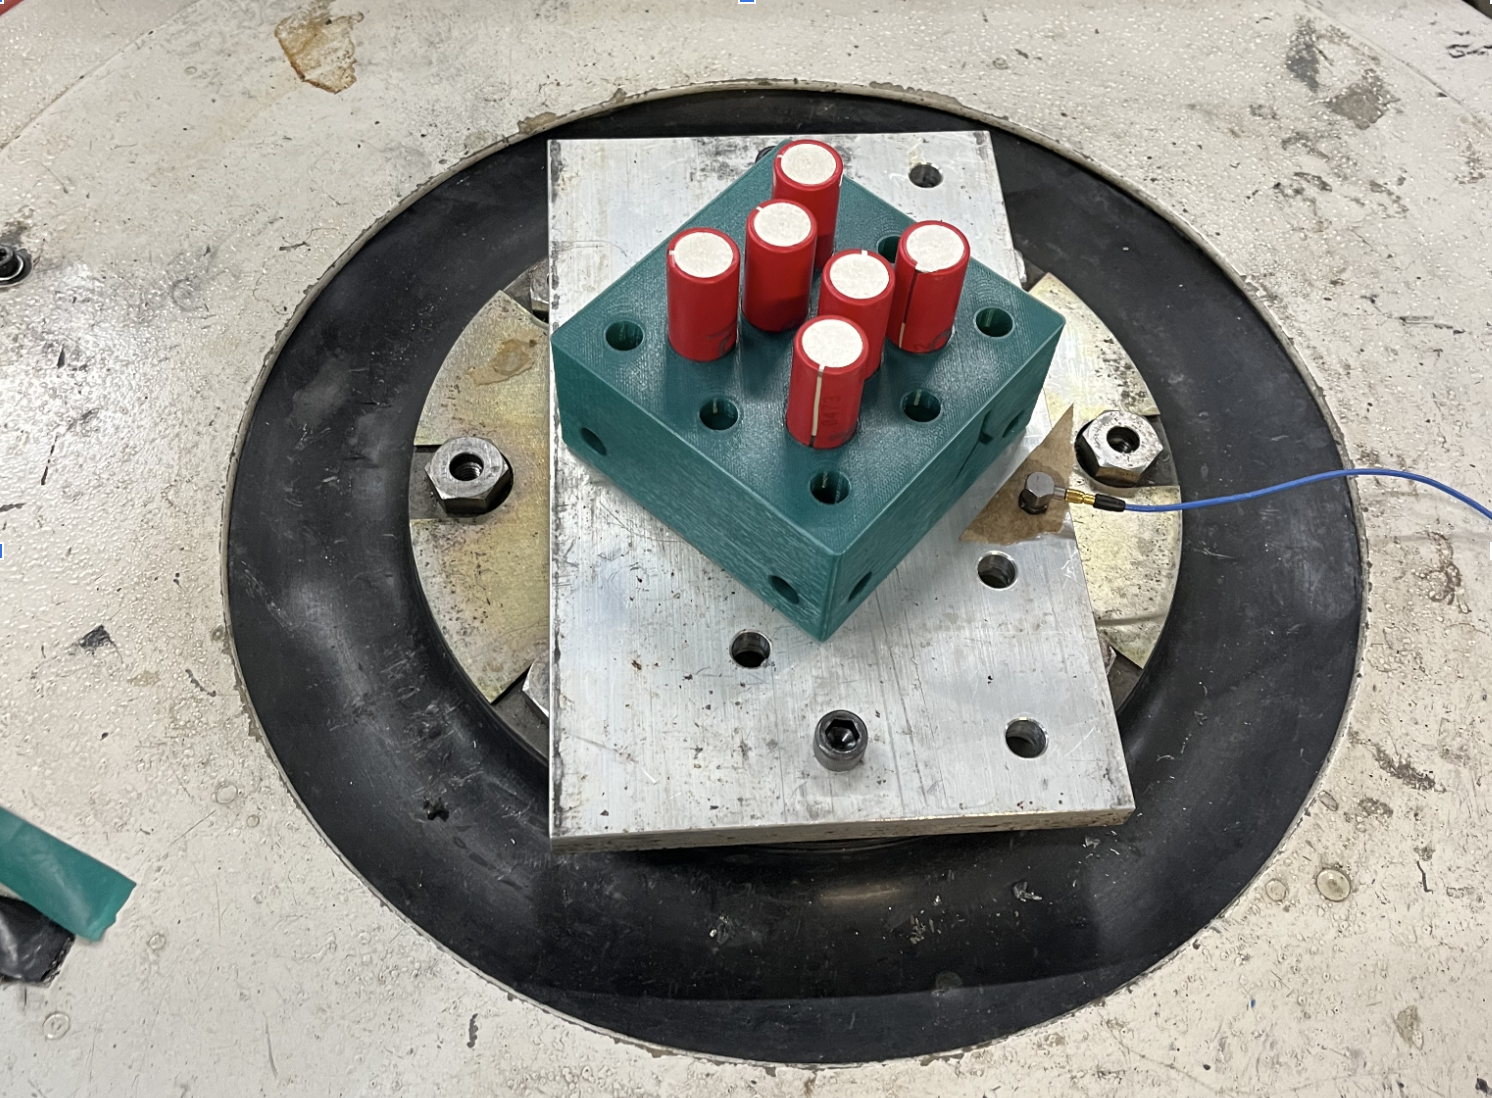
\includegraphics[width=\textwidth]{images/vibe-setup}
\caption{Six cells in the 3D printed battery holder, mounted to the Yokohama shaker table.}
\label{fig:cell-setup}
\end{figure}

\begin{table}[H]
    \centering
    \caption{Capacity and voltage measurements made before vibration testing.}
    \begin{tabular}{llll}
        \textbf{Cell \#} & \textbf{OCV before vibe (V)} & \textbf{Capacity before vibe (mAh)} & \textbf{Pass vibe visual inspection? y/n} \\ \hline
        1 & 4.14 & 3138 & y \\ 
        2 & 4.15 & 3100 & y \\ 
        3 & 4.15 & 3151 & y \\ 
        4 & 4.14 & 3132 & y \\ 
        5 & 4.16 & 3124 & y \\ 
        6 & 4.16 & 3099 & y \\ 
        7 & 4.14 & 3109 & y \\ 
        8 & 4.14 & 3091 & y \\ 
        9 & 4.15 & 3159 & y \\ 
        10 & 4.14 & 3148 & y \\ 
        11 & 4.17 & 3123 & y \\ 
        12 & 4.17 & 3102 & y \\ 
        13 & 4.13 & 3093 & y \\ 
        14 & 4.14 & 3091 & y \\ 
        15 & 4.15 & 3139 & y \\ 
        16 & 4.15 & 3158 & y \\ 
        17 & 4.17 & 3111 & y \\ 
        18 & 4.17 & 3103 & y \\ 
        19 & 4.13 & 3107 & y \\ 
        20 & 4.13 & 3110 & y \\ 
        21 & 4.14 & 3095 & y \\ 
        22 & 4.13 & 3116 & y \\ 
        23 & 4.15 & 3169 & y \\ 
        24 & 4.15 & 3141 & y \\ 
        25 & 4.15 & 3161 & y \\ 
        26 & 4.15 & 3162 & y \\ 
        27 & 4.17 & 3117 & y \\ 
        28 & 4.17 & 3109 & y \\ 
        29 & 4.17 & 3099 & y \\ 
        30 & 4.17 & 3126 & y \\ 
        31 & 4.14 & 3096 & y \\ 
        32 & 4.14 & 3065 & y \\ 
        33 & 4.14 & 3102 & y \\ 
        34 & 4.14 & 3119 & y \\ 
        35 & 4.15 & 3153 & y \\ 
        36 & 4.15 & 3142 & y \\ 
    \end{tabular}
    \label{tab:acc1}
\end{table}



\begin{table}[H]
    \centering
    \caption{Capacity and voltage measurements after vibration testing. The differences in measured capacity from before and after vibration shows that all cells passed the acceptance test.}
    \begin{tabular}{lllll}
        \textbf{Cell \#} & \textbf{OCV after vibe (V)} & \textbf{Capacity after vibe (mAh)} & \textbf{\%diff OCV} & \textbf{\%diff capacity} \\ \hline
        1 & 4.15 & 3117 & 0\% & 1\% \\ 
        2 & 4.15 & 3110 & 0\% & 0\% \\ 
        3 & 4.15 & 3108 & 0\% & 1\% \\ 
        4 & 4.14 & 3163 & 0\% & -1\% \\ 
        5 & 4.16 & 3191 & 0\% & -2\% \\ 
        6 & 4.16 & 3179 & 0\% & -3\% \\ 
        7 & 4.14 & 3169 & 0\% & -2\% \\ 
        8 & 4.14 & 3168 & 0\% & -2\% \\ 
        9 & 4.15 & 3123 & 0\% & 1\% \\ 
        10 & 4.15 & 3124 & 0\% & 1\% \\ 
        11 & 4.17 & 3111 & 0\% & 0\% \\ 
        12 & 4.17 & 3114 & 0\% & 0\% \\ 
        13 & 4.14 & 3125 & 0\% & -1\% \\ 
        14 & 4.14 & 3183 & 0\% & -3\% \\ 
        15 & 4.14 & 3131 & 0\% & 0\% \\ 
        16 & 4.15 & 3142 & 0\% & 1\% \\ 
        17 & 4.17 & 3141 & 0\% & -1\% \\ 
        18 & 4.17 & 3121 & 0\% & -1\% \\ 
        19 & 4.14 & 3103 & 0\% & 0\% \\ 
        20 & 4.13 & 3121 & 0\% & 0\% \\ 
        21 & 4.14 & 3168 & 0\% & -2\% \\ 
        22 & 4.14 & 3140 & 0\% & -1\% \\ 
        23 & 4.15 & 3101 & 0\% & 2\% \\ 
        24 & 4.15 & 3132 & 0\% & 0\% \\ 
        25 & 4.15 & 3146 & 0\% & 0\% \\ 
        26 & 4.15 & 3141 & 0\% & 1\% \\ 
        27 & 4.17 & 3161 & 0\% & -1\% \\ 
        28 & 4.17 & 3164 & 0\% & -2\% \\ 
        29 & 4.17 & 3168 & 0\% & -2\% \\ 
        30 & 4.17 & 3176 & 0\% & -2\% \\ 
        31 & 4.14 & 3180 & 0\% & -3\% \\ 
        32 & 4.14 & 3154 & 0\% & -3\% \\ 
        33 & 4.14 & 3111 & 0\% & 0\% \\ 
        34 & 4.14 & 3118 & 0\% & 0\% \\ 
        35 & 4.15 & 3105 & 0\% & 2\% \\ 
        36 & 4.15 & 3114 & 0\% & 1\% \\ 
    \end{tabular}
    \label{tab:acc2}
\end{table}

\section{Welding Process Specification}

\subsection{Equipment}

The battery welder used is a kit welder\footnote{\url{https://malectrics.eu/product/diy-arduino-battery-spot-welder-prebuilt-kit-v3/}} powered by a 12000mAh 3S LiPo battery. The full welding setup including battery, weld controller, and probes can be seen in Fig.~\ref{fig:welder}. Detailed information about the welding equipment is shown in Table~\ref{tab:weldequip}. 

Not every detail from the \textit{\textbf{PRC-0009 Rev. D}} spec is able to be replicated with this setup, including the ability to measure the down force of the probes on to working surface. In order to make sure that the welds stay consistent, a \textit{trained hand} method is used. This ensures that the person performing the resistance spot welds on the flight cells is the same person performing the welds for the weld process verification. In both scenarios this person is Matt Ruffner.

\begin{figure}[h!]
\centering
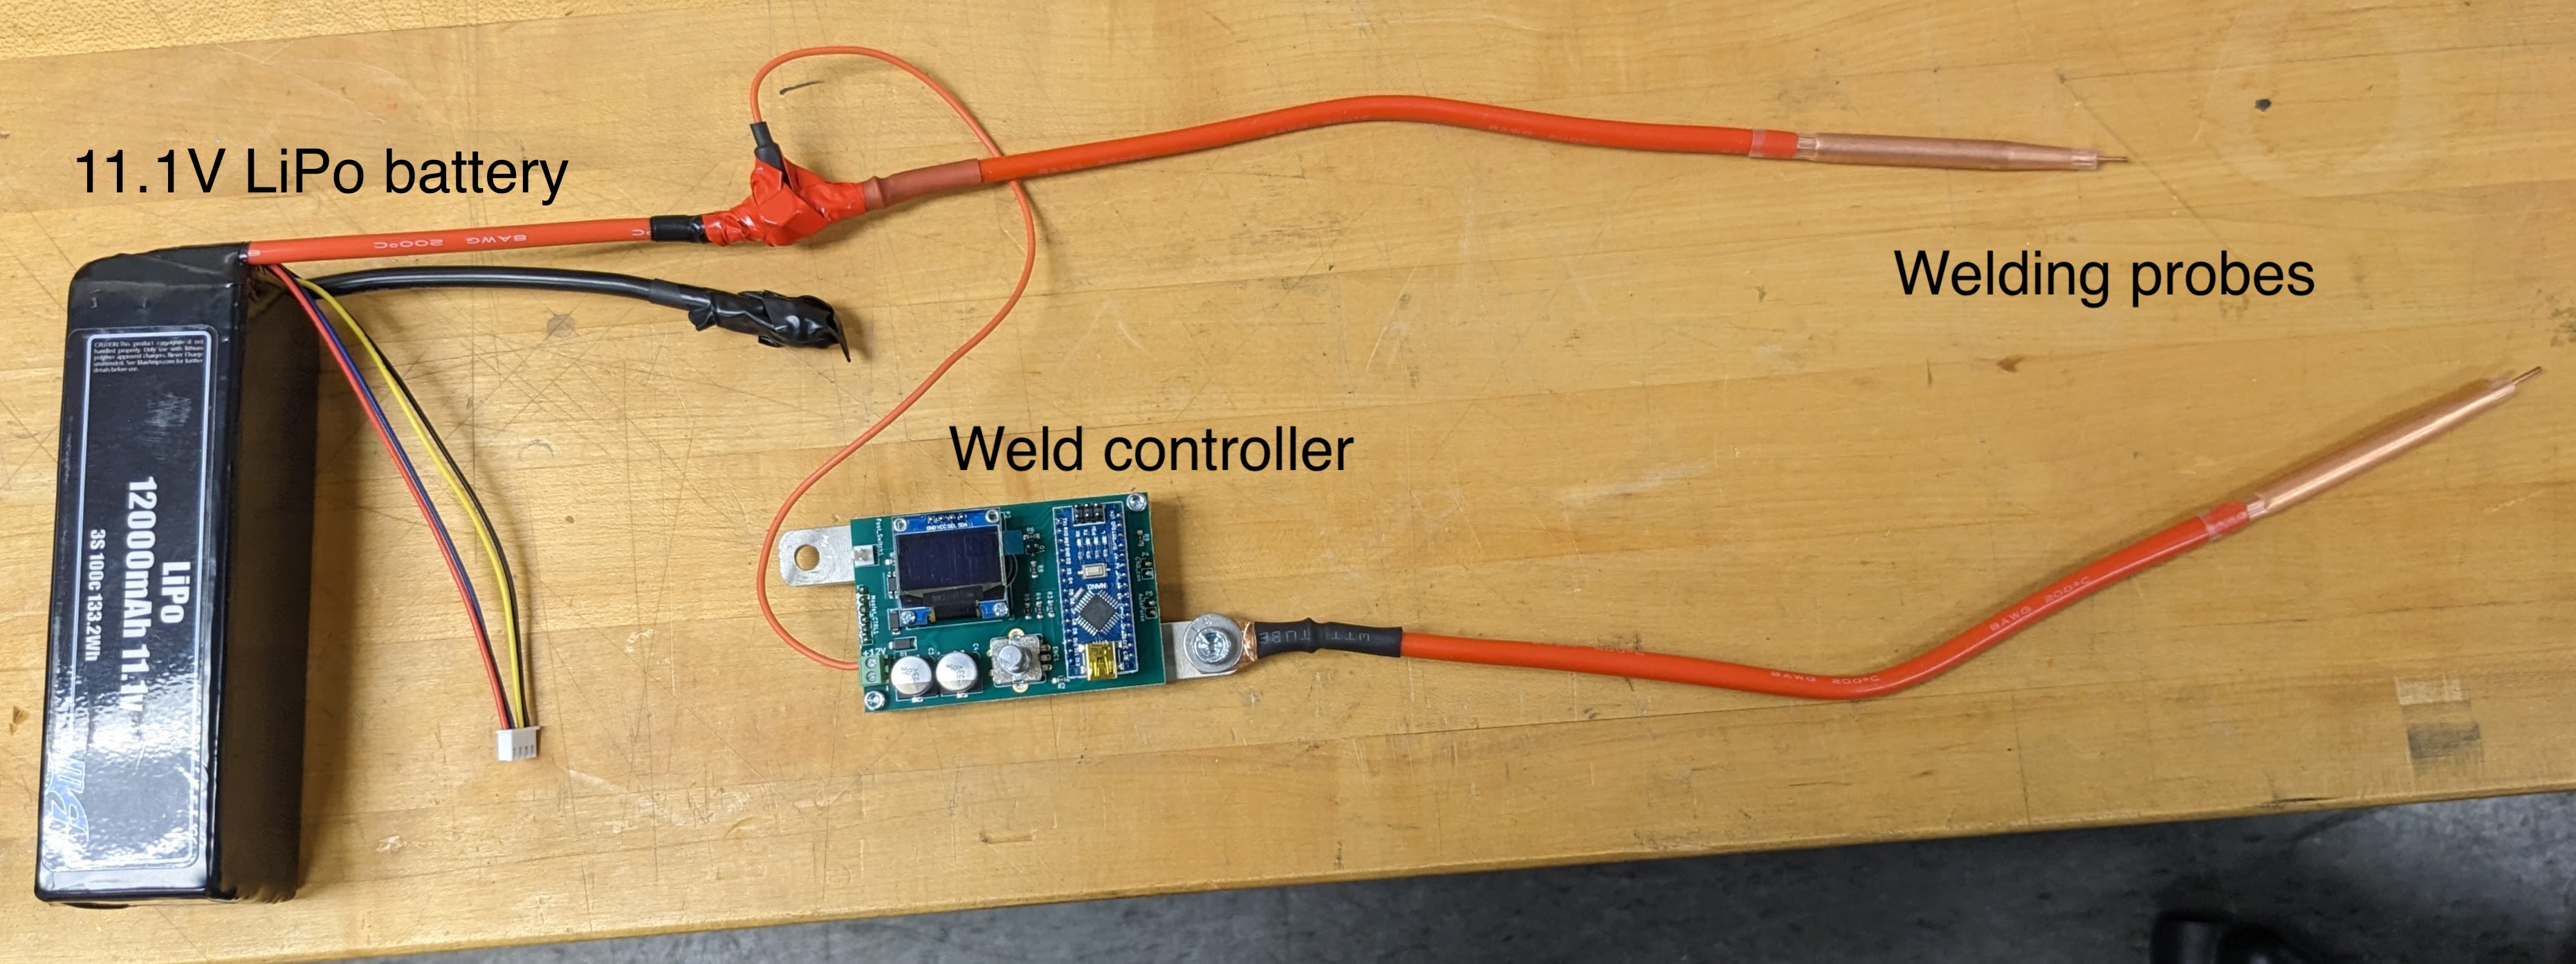
\includegraphics[width=\textwidth]{images/welder}
\caption{Battery tab welding equipment. Battery (left) attaches to the weld controller (center) and allows weld parameters to be changed for use with the welding probes (right).}
\label{fig:welder}
\end{figure}


\begin{table}
\centering
\caption{Resistance spot welding weld schedule}
\label{tab:weldequip}
\begin{tabular}{|l l|}
\hline
\multicolumn{2}{|l|}{\textbf{Equipment Identification}} \\
Owner / location &  KRUPS, RGAN 110 \\
Power supply & MaxAmps 3S 12000 mAh LiPo \\
Weld controller serial number & sw-pbkit-v4 \\
Weld head / model & SeeSii 2021 \\
Interconnecting cable & 8 AWG, 6 in \\
&\\
\hline
\multicolumn{2}{|l|}{\textbf{Battery}} \\
Manufacturer & Sanyo \\
Type / size & NCR18650B-H07XA \\
Material type & Lithium ion battery \\
&\\
\hline
\multicolumn{2}{|l|}{\textbf{Connecting Material}} \\
Manufacturer & SeeSii \\
Type & Nickel \\
Thickness / width & 1.5"L x 0.355"W x 0.005"T \\
&\\
\hline
\multicolumn{2}{|l|}{\textbf{Electrodes}} \\
Manufacturer & SeeSii \\
Material & Copper \\
Distance between electrode tips & 0.2 in \\
Contact tip surface shape & round \\
Electrode tip size & 0.059 in. diameter\\
&\\
\hline
\multicolumn{2}{|l|}{\textbf{Welding electrode configuration and setup}} \\
Number of pulses &  1 \\
%Squeeze time      & 1 second \\
%Upslope duration & N/A \\
Pulse duration & 10 ms \\
%Downslope & 0 ms \\
%Hold time & 500 ms \\
%Negative Electrode Force &1 lbs \\
%Positive Electrode Force &1 lbs\\
%Pull force & ??\\
\hline
\end{tabular}
\end{table}

\subsection{Process}

say certified operator instead of trained hand

add reference to section 4 table

A tab weld consists of two separate weld instances, yielding 4 weld points, or ``nuggets", on each tab. There are two types of packs required for this mission. The 3S1P pack requires standard tab-to-battery welds, while the 1S3P pack requires tab-to-battery welds as well as tab-to-tab welds.

To qualify both of these processes, plug pull out tests will be done for tabs attached to other tabs and tabs attached to batteries. In both scenarios, success is determined by plug pullout, signifying that the weld is indeed stronger than the original material by itself.



\begin{enumerate}
\item Cut 4 pieces of tab material 1.5" long
\item Mark 4 points 0.2 in apart to weld at on each tab
\item Ensure the battery powering the welder is charged and its voltage is greater than 11.1 V
\item Initialize the weld controller and select 10ms weld pulse duration
\item Stabilize the battery and pin the tab with one electrode
\item Press the other weld tip to the battery
\item Repeat weld for second weld on a given tab. 
\end{enumerate}


\section{Weld Verification}

change language to "it can be seen"

As per PRC-0009, 15 sets of example welds are the minimum test batch size. To this end, tabs were attached to both the positive and negative ends of two Sanyo cells. There are 16 total welds resulting (in groups of 4 spot welds for each tab attachment point).

Figure~\ref{fig:stabilized-tab} shows a tab sitting on top of the first cell, prior to tabbing. After this, 4 points were marked on the tab to indicated where the welds were to be placed. After the markings are placed, the weld tips are pressed to the tab with a moderate amount of force by hand. The weld controller senses this connection and triggers a weld 4 seconds after the tips are touched to the tab. After both welds have been done on a single tab (producing 4 weld nuggets), the tab looks like that shown in Fig.~\ref{fig:post-weld}.

\begin{figure}[h]
\centering
\includegraphics[width=12cm]{images/stabilized-tab}
\caption{Nickel tab stabilized on top to cell prior to welding.}
\label{fig:stabilized-tab}
\end{figure}

\begin{figure}[h]
\centering
\begin{subfigure}{0.6\textwidth}
\includegraphics[width=\textwidth]{images/post-weld}
\caption{After both welds have been performed on the tab. You can see the silver sharpie locater markings underneath the weld to help guide the placement of the weld tips during the welding process.}
\label{fig:post-weld}
\end{subfigure}
\hfill
\begin{subfigure}{0.3\textwidth}
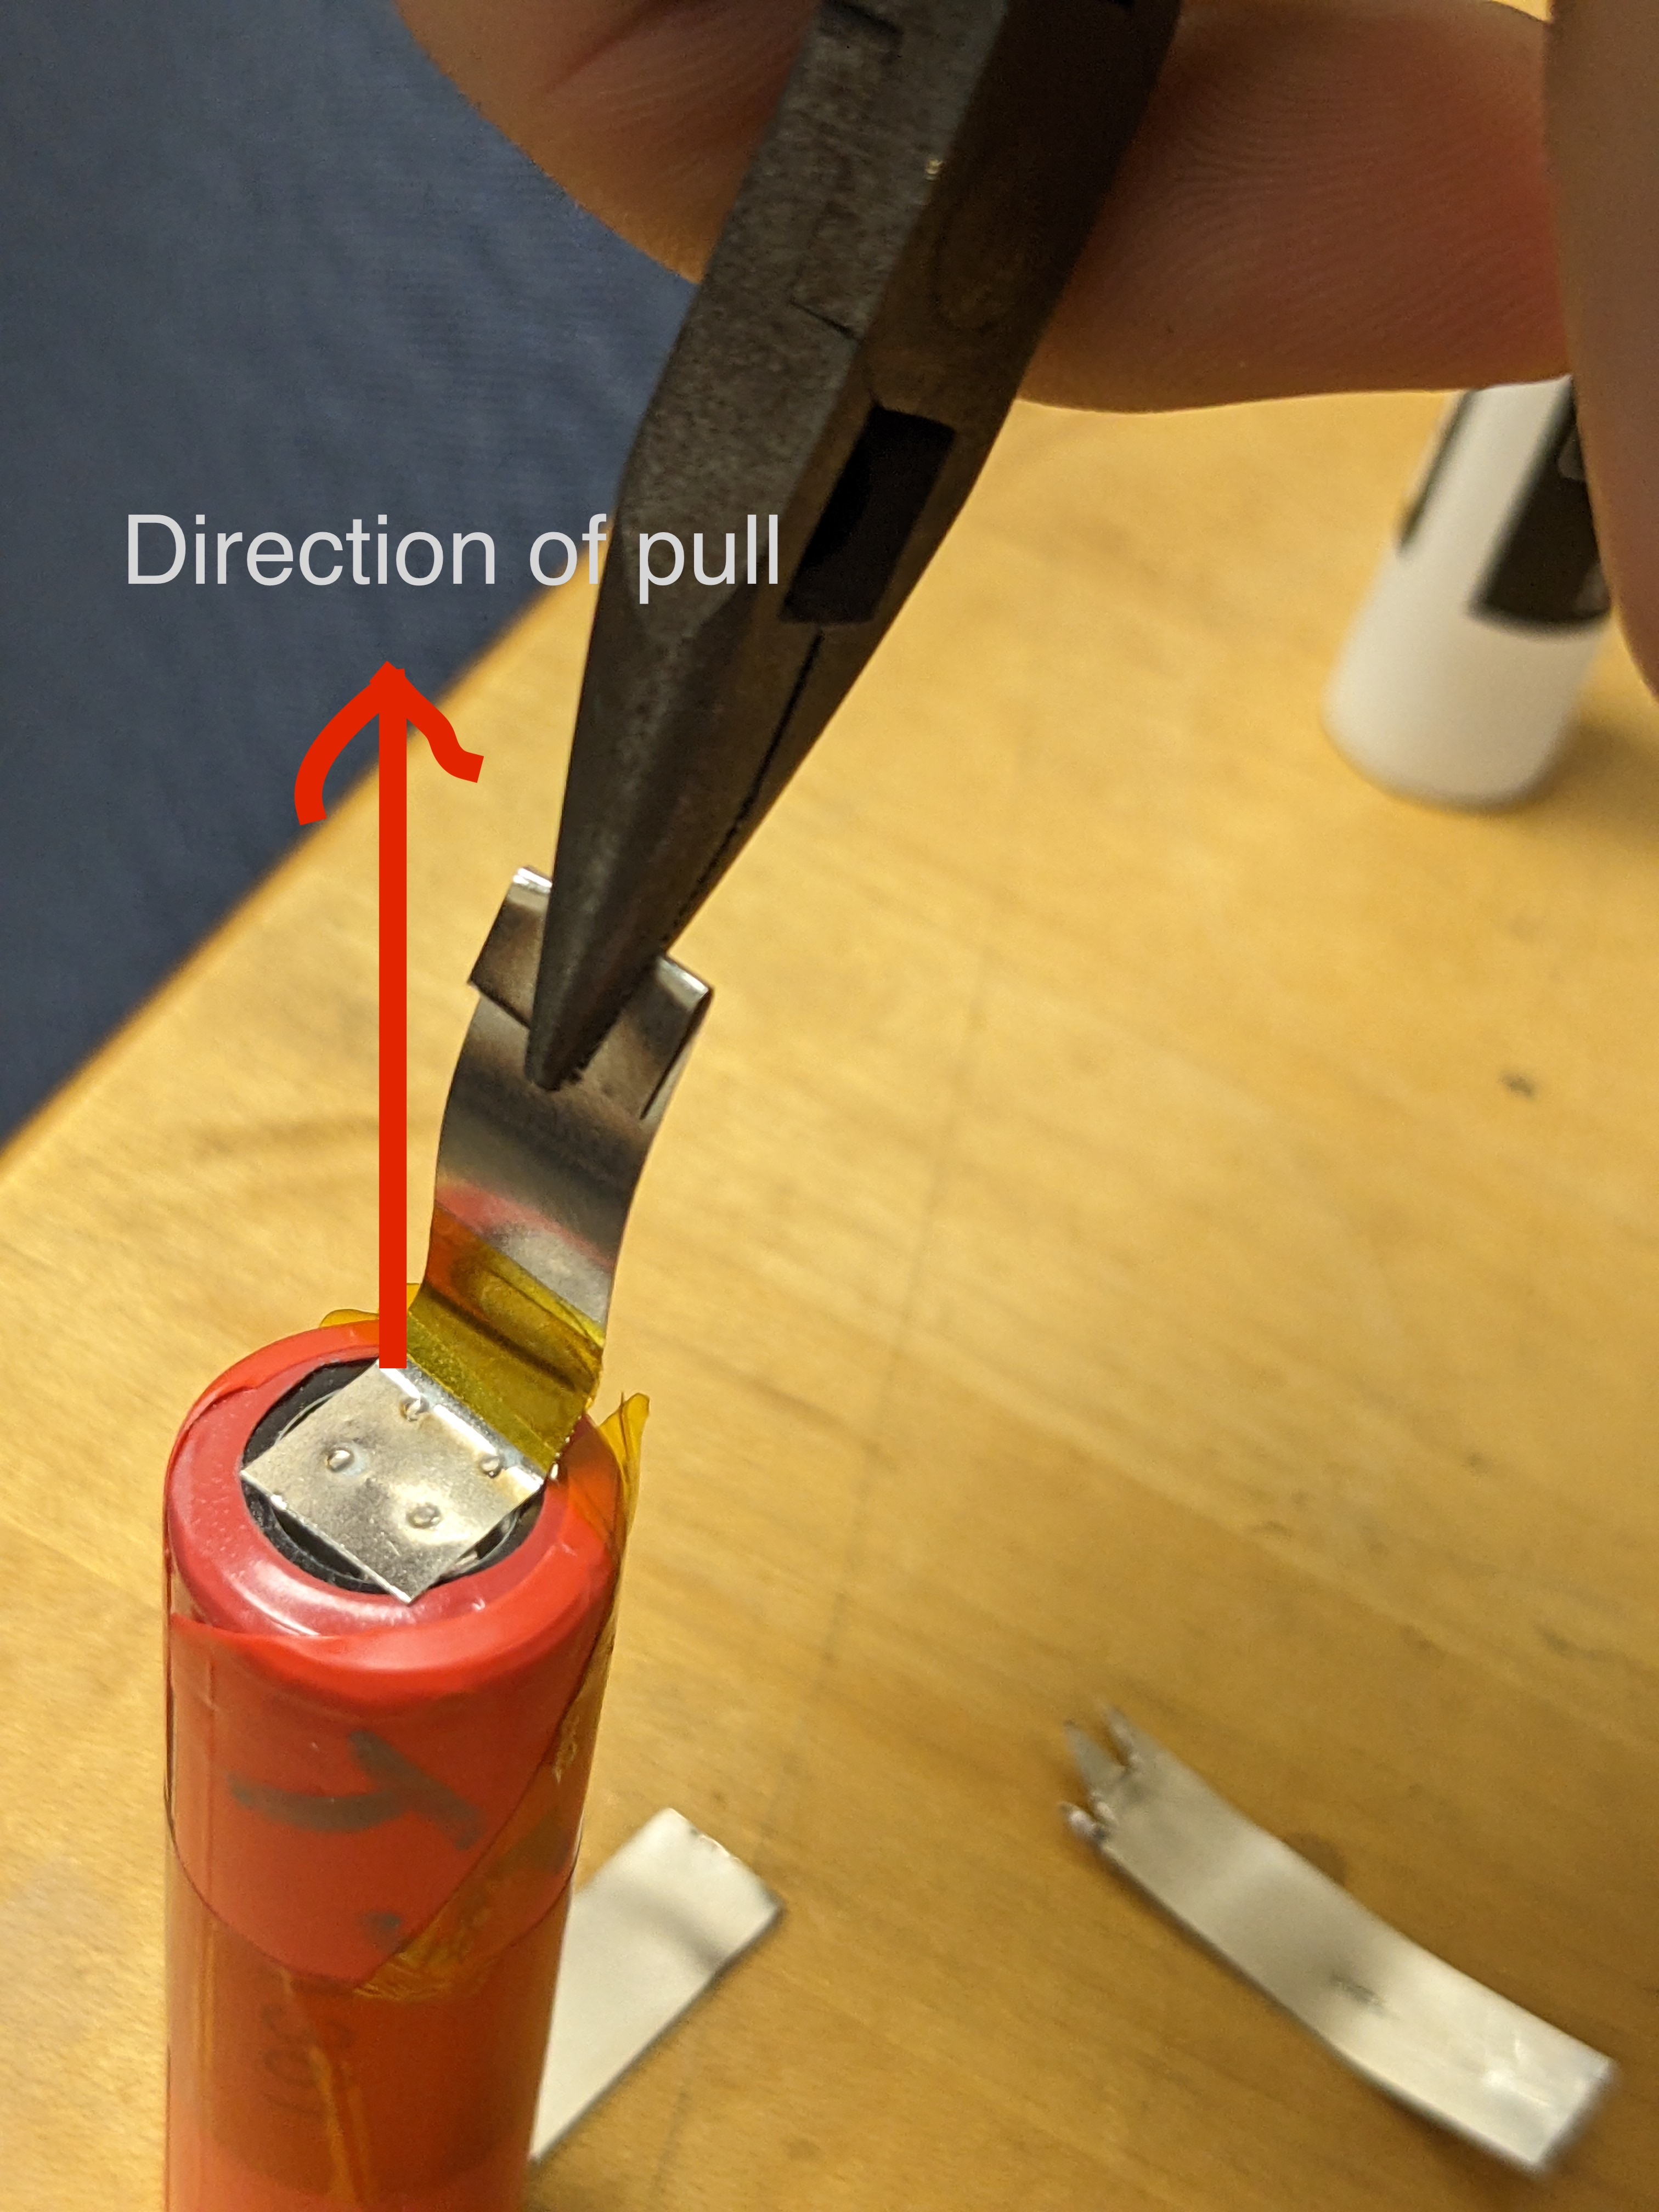
\includegraphics[width=\textwidth]{images/direction-of-pull}
\caption{Pliers were used to pull the welded tab off of the battery at a right angle to the surface of the weld.}
\label{fig:pull-config}
\end{subfigure}
\caption{Result of resistance spot welding using our weld controller and the configuration of the destructive peel test.}
\end{figure}


After all 4 tabs are attached to the two cells with a total of 16 weld nuggets, the peel test proceeds. The peel test consists of holding the cell in the upright position and using a pair of pliers to pull the tab at a 90 degree angle to the working surface (the plane of the welds). This configuration is shown in Fig.~\ref{fig:pull-config}.




Using this configuration, the destructive peel test continued. The tabs were pulled at right angles until the tab cam free from the battery. The results of the 4 peel tests are shown in Figs.~\ref{fig:peel-1}, \ref{fig:peel-2}, \ref{fig:peel-3}, and \ref{fig:peel-4}. As you can see, all 16/16 weld nuggets proved stronger than the tab, and the 4 peel tests resulted in 100\% plug pullout. 



\begin{figure}[H]
\centering

\begin{subfigure}{0.3\textwidth}
\includegraphics[width=\textwidth]{images/tpo-1}
\caption{Tab 1, test cell 1.}
\label {fig:peel-1}
\end{subfigure}
\hfill
\begin{subfigure}{0.3\textwidth}
\includegraphics[width=\textwidth]{images/tpo-2}
\caption{Tab 2, test cell 1.}
\label {fig:peel-2}
\end{subfigure}
\\
\begin{subfigure}{0.3\textwidth}
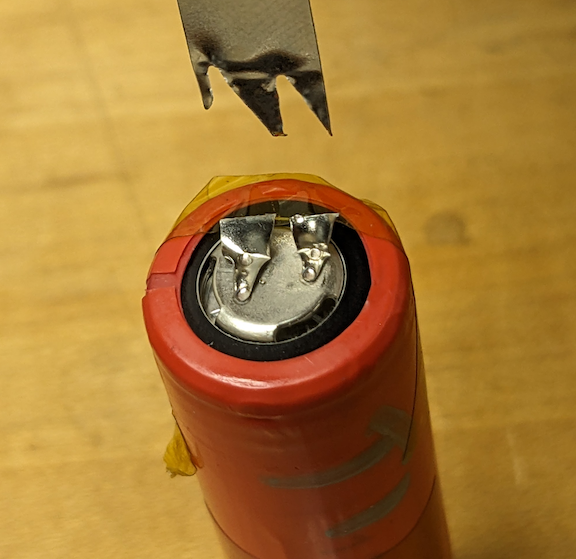
\includegraphics[width=\textwidth]{images/tpo-3}
\caption{Tab 1, test cell 2.}
\label {fig:peel-3}
\end{subfigure}
\hfill
\begin{subfigure}{0.3\textwidth}
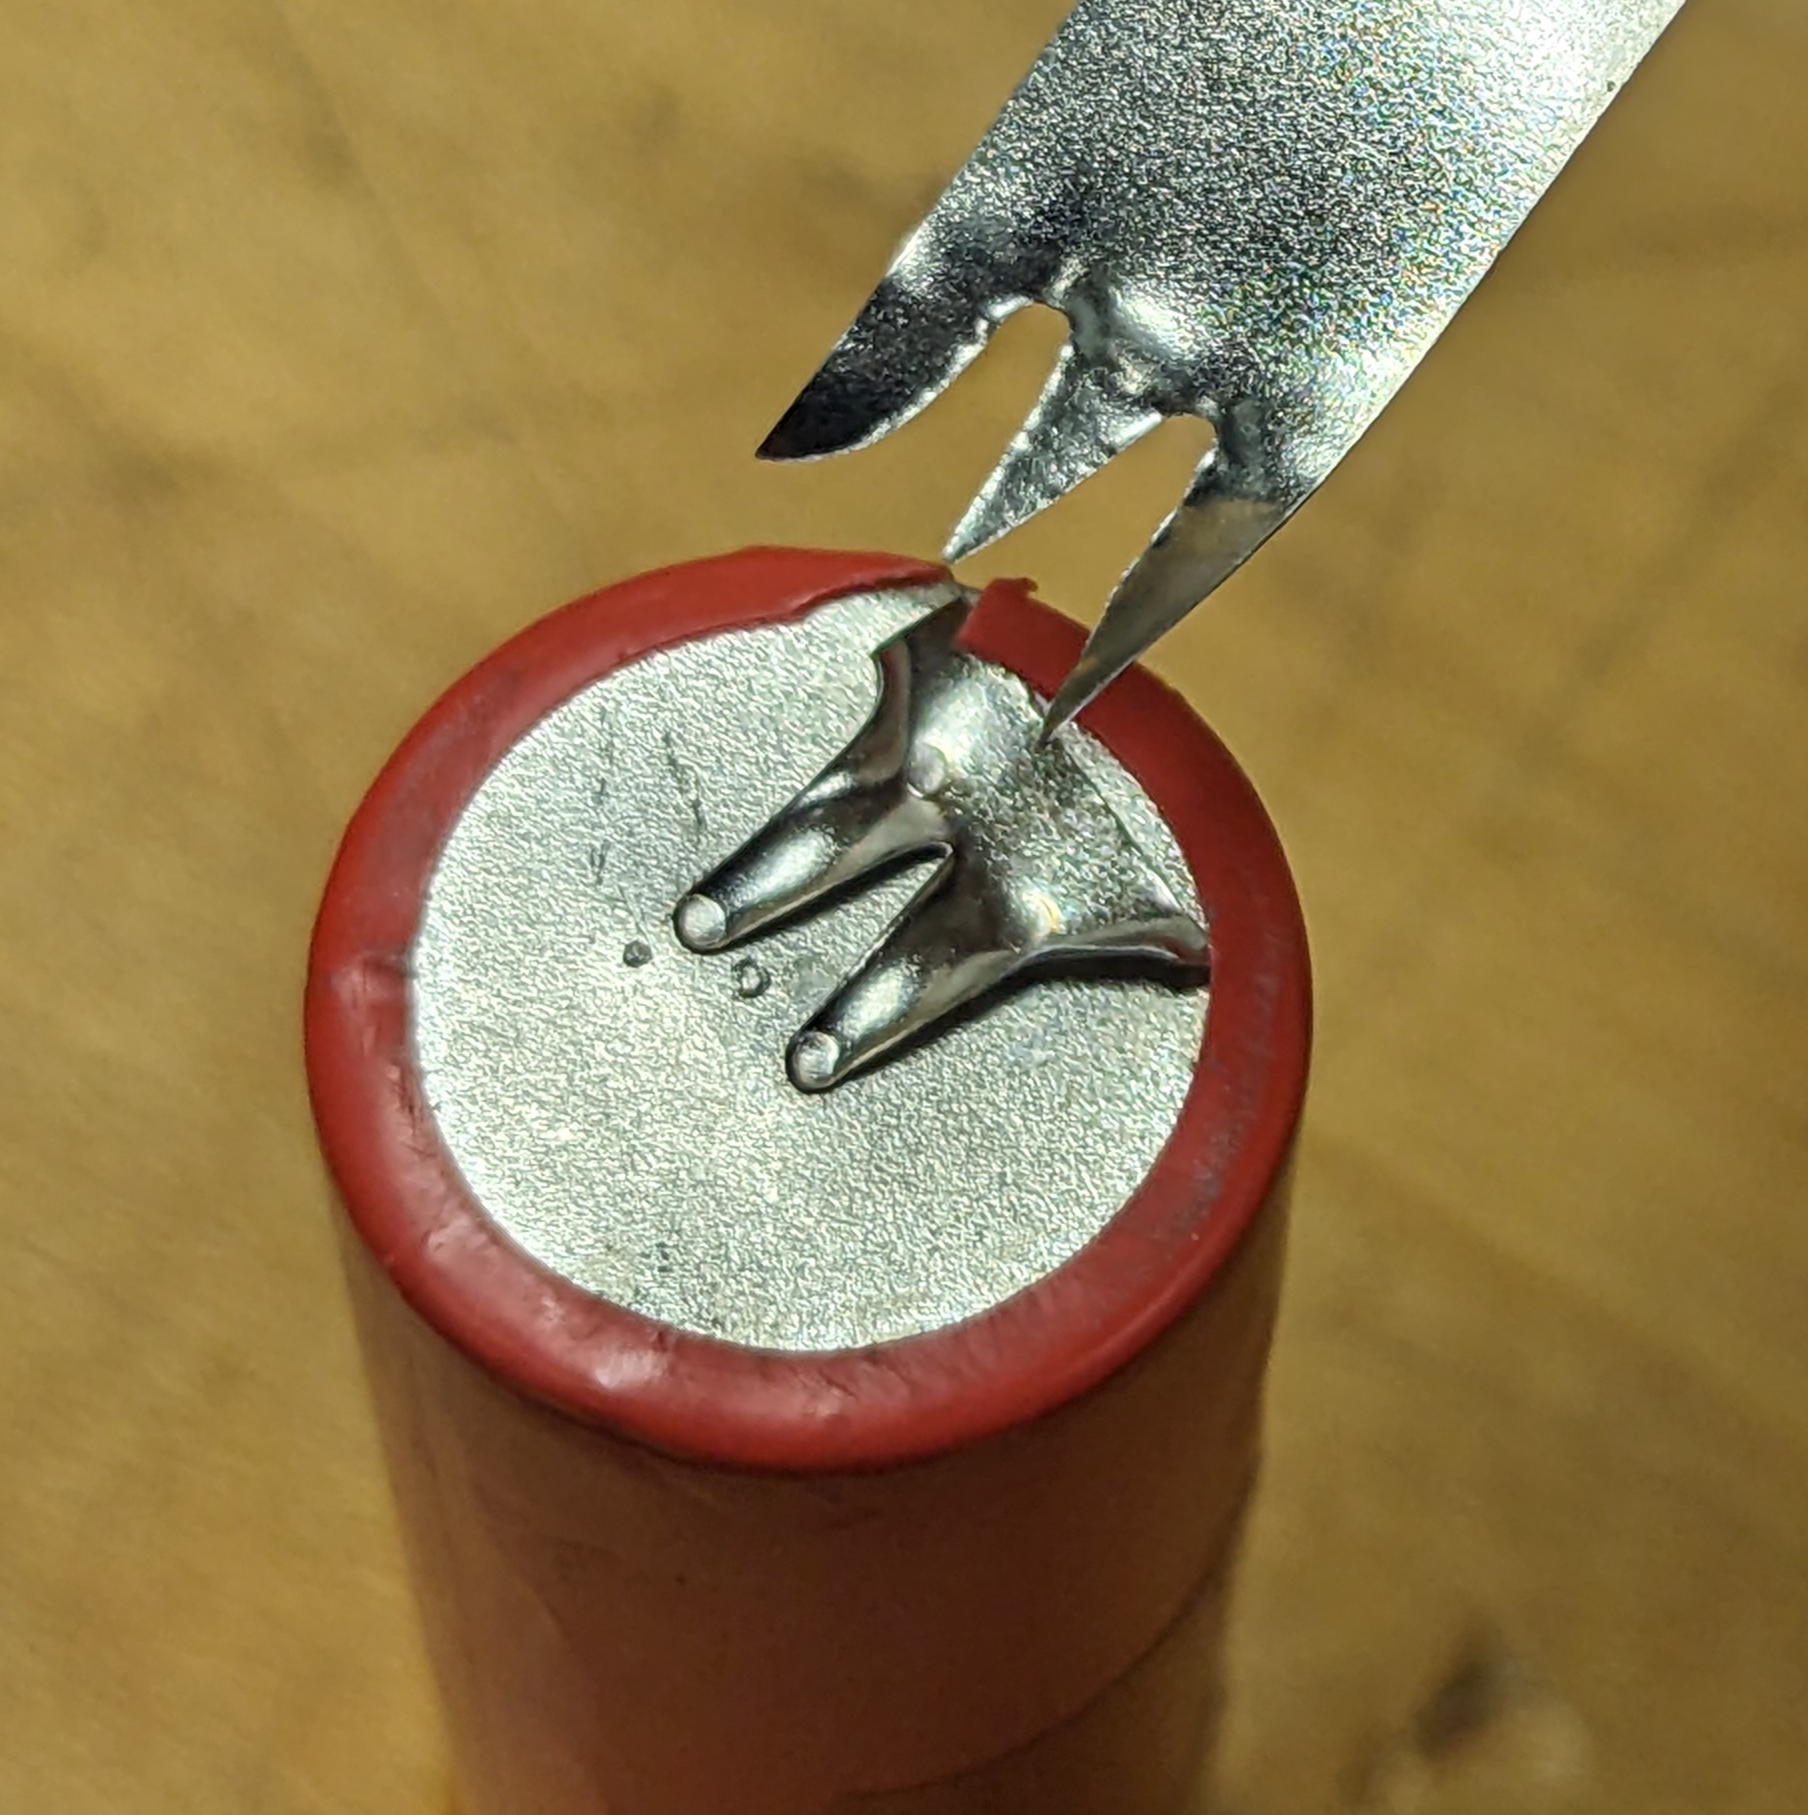
\includegraphics[width=\textwidth]{images/tpo-4}
\caption{Tab 2, test cell 2.}
\label {fig:peel-4}
\end{subfigure}
\caption{Results of plug pull out tests on the sample batch of welds.}
\end{figure}

\subsection{Weld Process Verification Summary}
Using the welding setup shown in Fig.~\ref{fig:welder}, 16 weld nuggets were created and tested to destruction with a peel test. For all 16 nuggets, plug pullout occurred. This confirms the strength of the welding process specified in this document.

\section{Battery Tabbing Arrangement}

The KREPE-2 capsules have 2 battery packs with 3 cells each. One is a 3.7V pack with the cells tabbed in parallel, and another 11.1V pack with the cells tabbed in series. Figures \ref{fig:parallel-pack} and \ref{fig:series-pack} show the arrangement of the tabs on the cells for the 3.7V and 11.1V pack, respectively.

\begin{figure}[H]
\centering

\begin{subfigure}{0.45\textwidth}
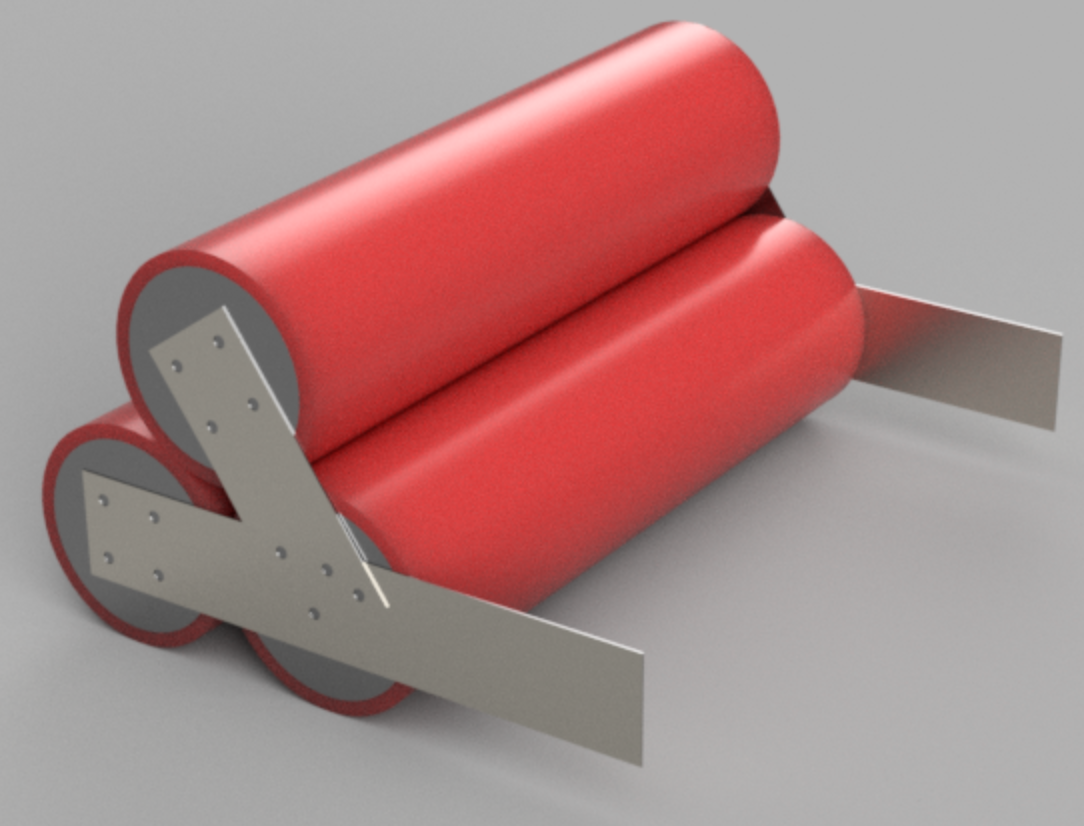
\includegraphics[width=\textwidth]{images/3p1s-battery-pack-render.png}
\caption{Rendering of 3.7V 3P1S battery pack}
\label {fig:parallel-pack}
\end{subfigure}
\hfill
\begin{subfigure}{0.45\textwidth}
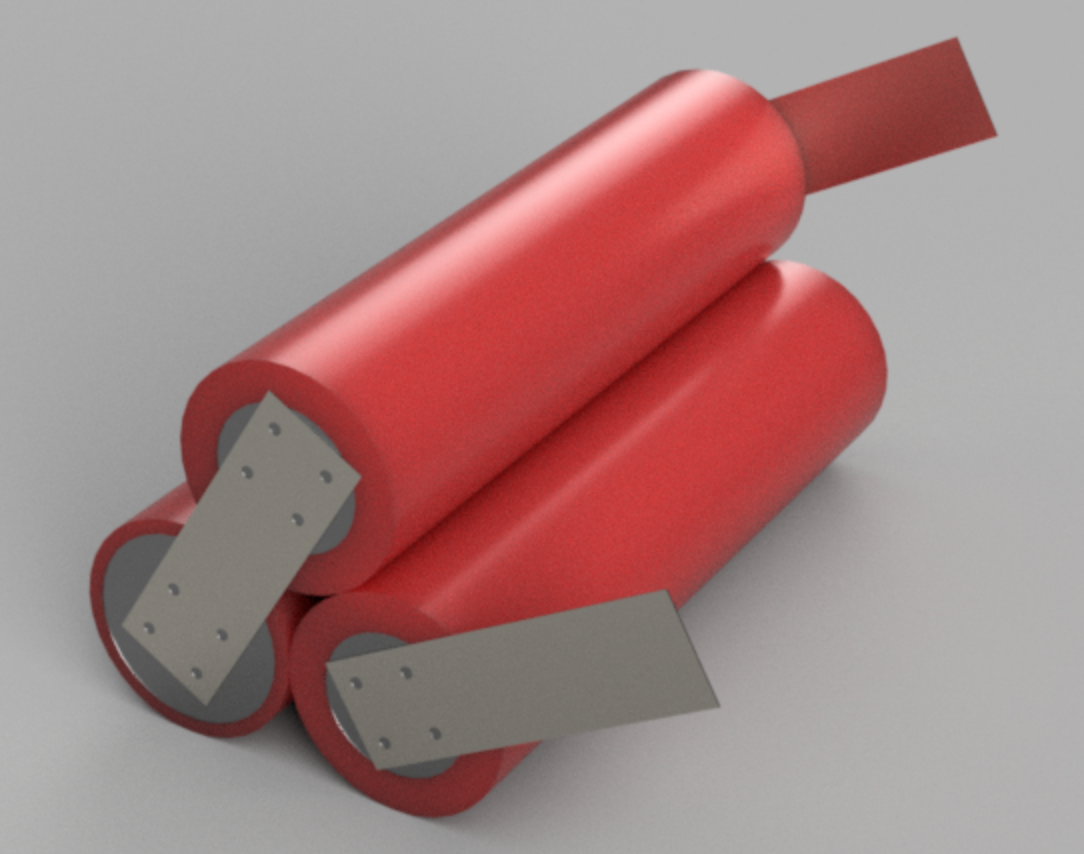
\includegraphics[width=\textwidth]{images/1p3s-battery-pack-render.png}
\caption{Rendering of 11.1V 1P3S battery pack}
\label {fig:series-pack}
\end{subfigure}

\end{figure}

The tabbing material is made of nickel strips measuring $0.005$ inches thick and $0.355$ inches wide and cut to length before being attached to the batteries. Dimensional drawings showing weld spacing and tab dimensions for both packs can be found in Figs. \ref{fig:1s3p_drawing} and \ref{fig:3s1p_drawing}.

\appendix

add drawing number

add approval for drawings

\section{Battery Pack Drawings}
Dimensions in inches.
\begin{figure}
\centering
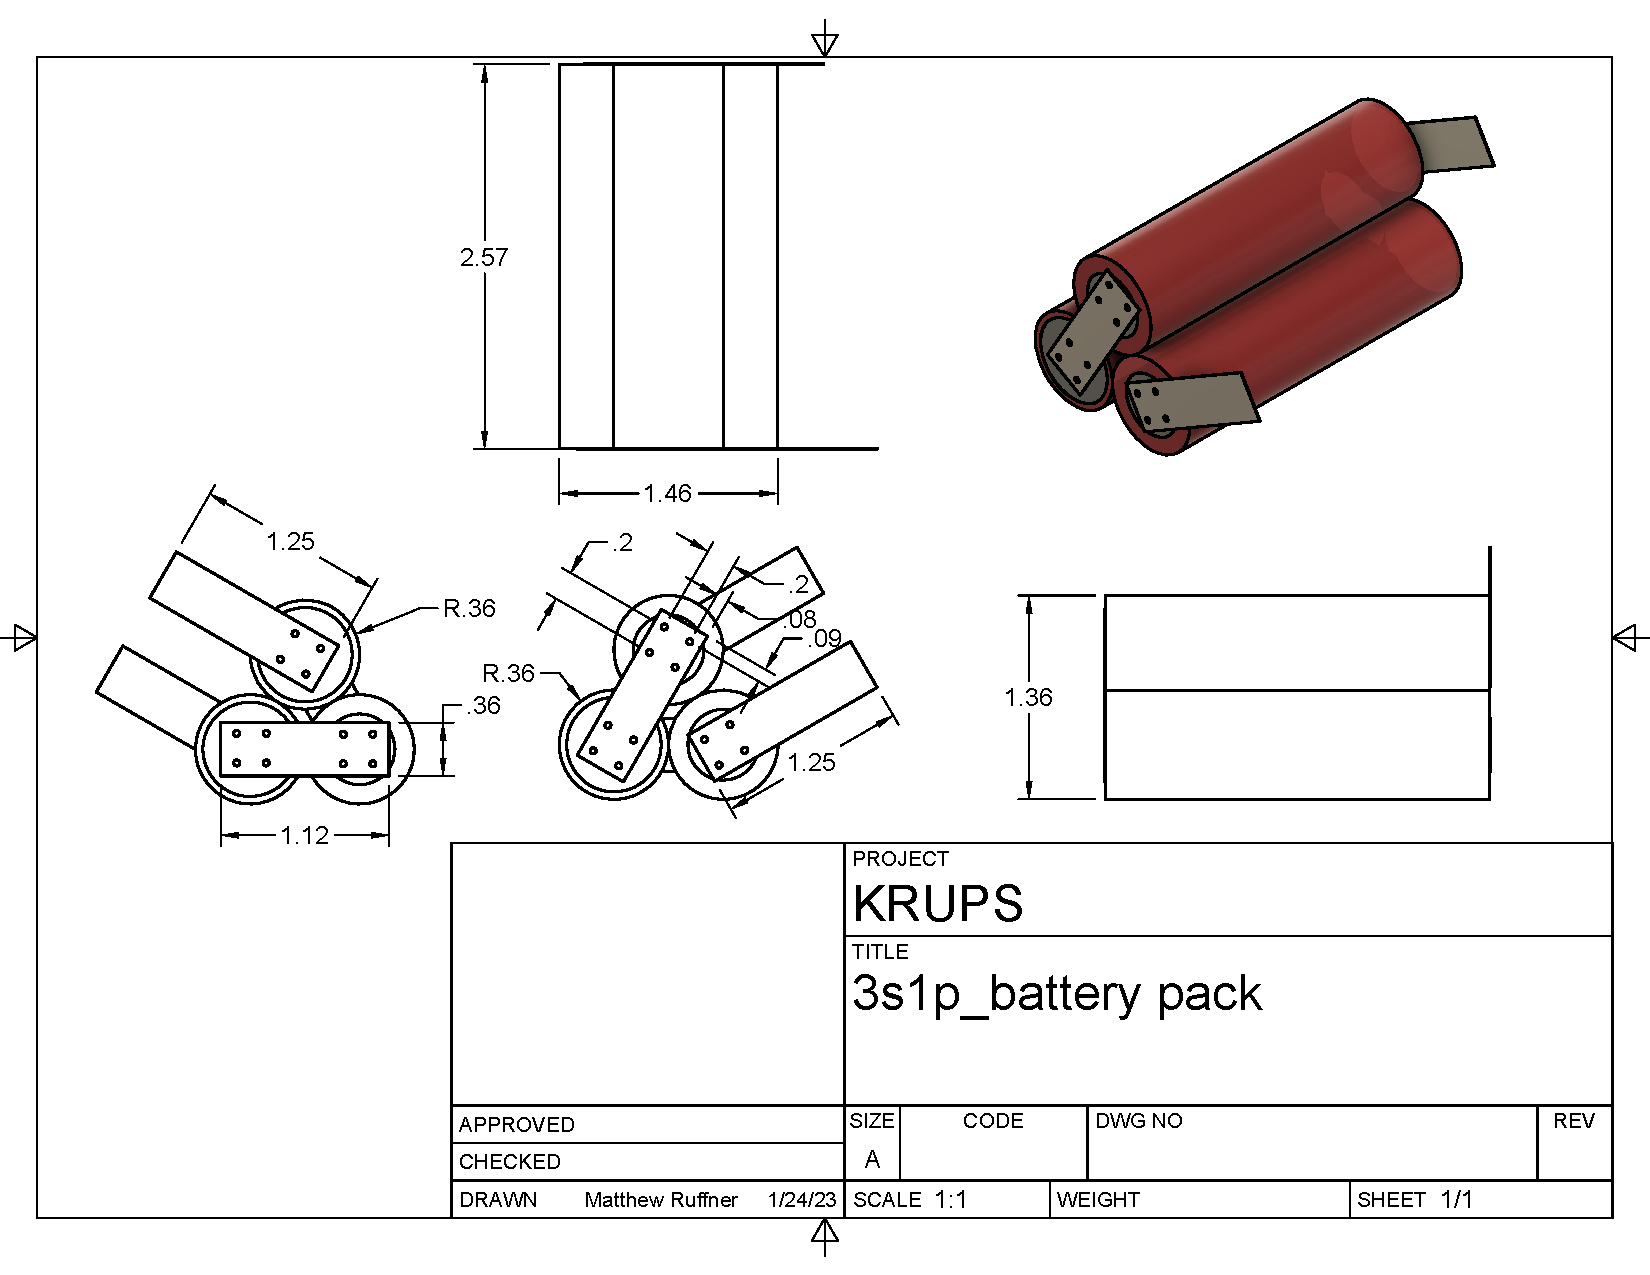
\includegraphics[width=\textwidth]{images/3s1p_battery pack Drawing v2.pdf}
\caption{3S1P pack drawing.}
\label{fig:3s1p_drawing}
\end{figure}

\begin{figure}
\centering
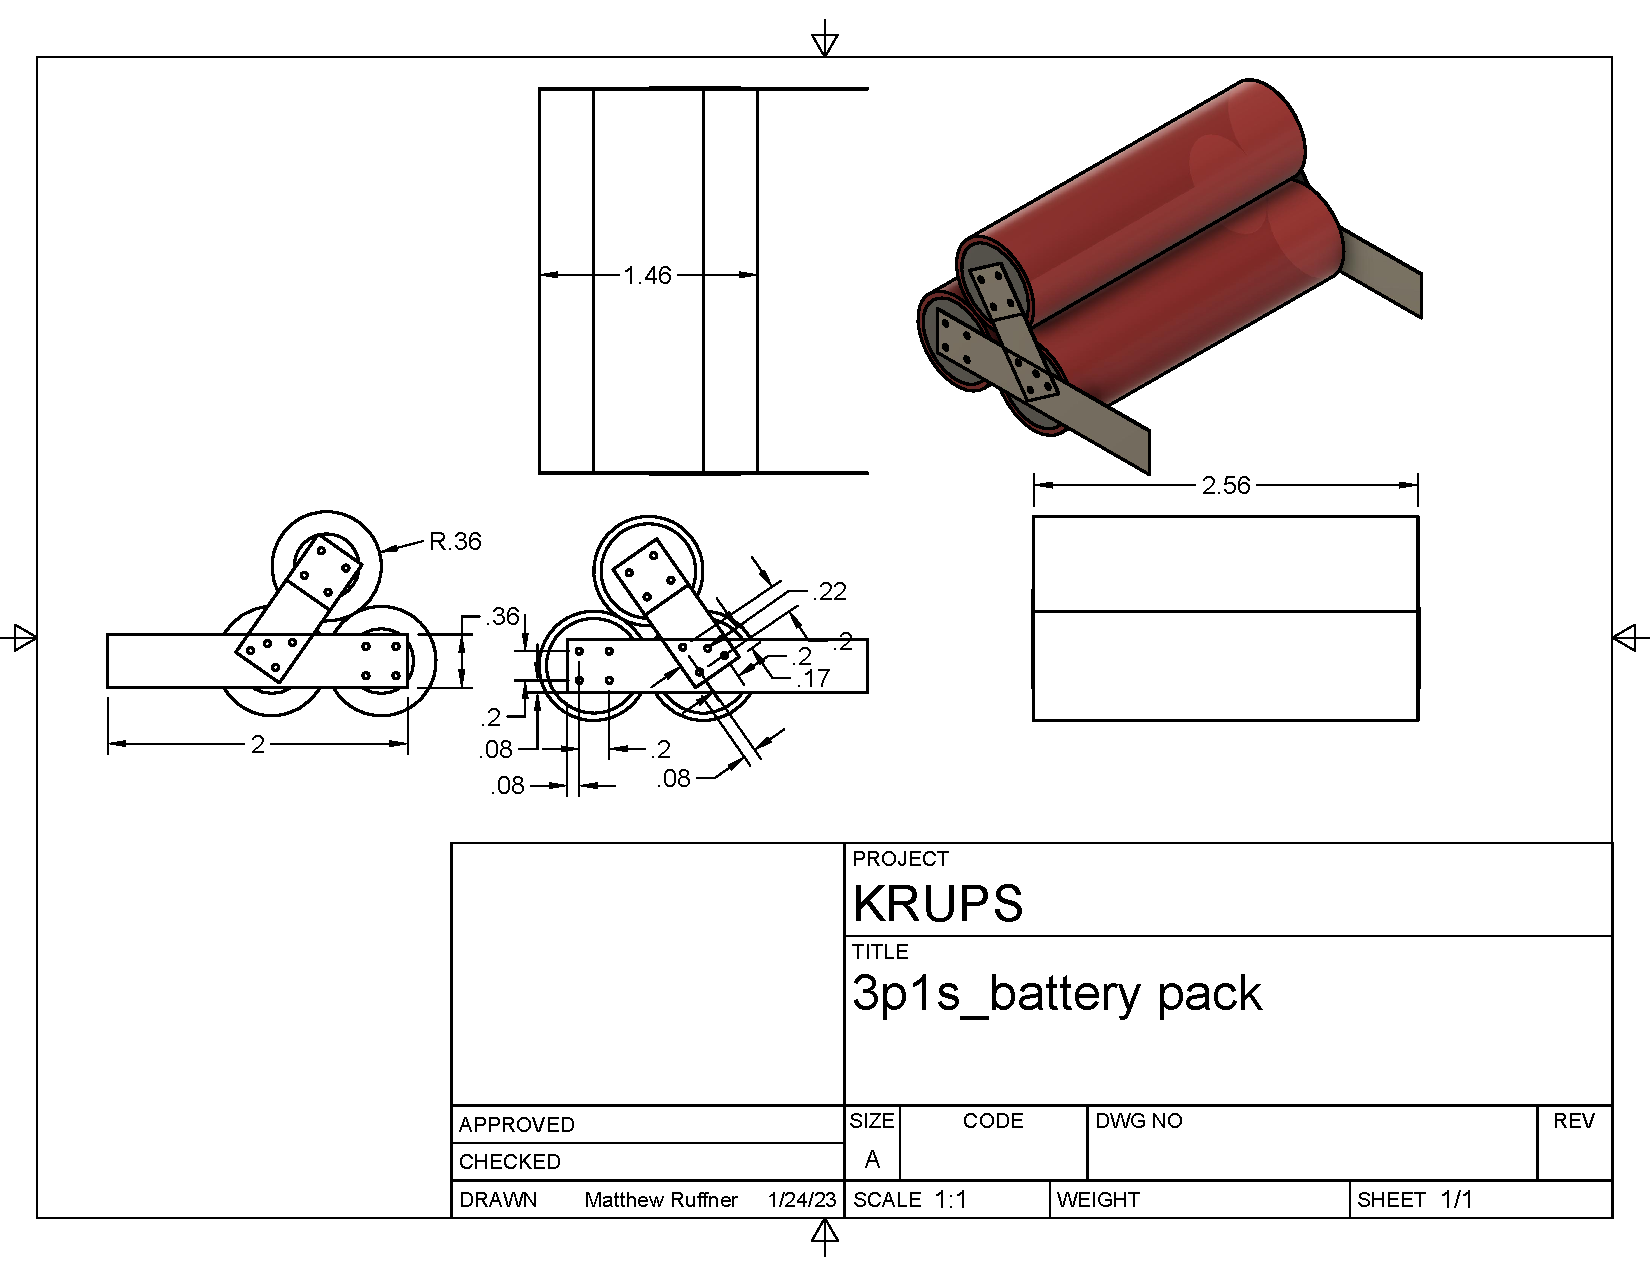
\includegraphics[width=\textwidth]{images/3p1s_battery pack Drawing v0.pdf}
\caption{1S3P pack drawing.}
\label{fig:1s3p_drawing}
\end{figure}



\end{document}

